\chapter{Implementation}\thispagestyle{empty} %chapter head
\graphicspath{{Chapter4/figures/}}
{\setstretch{1.5}


The implementation phase of LungInsight translates the proposed multimodal explainable AI
framework into a fully functional lung cancer prediction system. This chapter documents the
concrete steps taken to build, integrate, and validate each component of the pipeline—from
environment configuration and data ingestion through model training, explainability generation,
and clinical dashboard deployment.

\section{Introduction}

The implementation phase focused on realising the design of the LungInsight framework as a
working system capable of predicting lung cancer malignancy probability and disease stage from
CT imaging and structured clinical data. The primary objectives guiding this phase were: (i)
constructing a robust, reproducible data preprocessing pipeline for heterogeneous multimodal
inputs; (ii) implementing and training a DenseNet-based imaging branch fused with an MLP
clinical branch; (iii) integrating Grad-CAM and SHAP to produce patient-level explanations; and
(iv) deploying an interactive clinical decision-support dashboard.

\section{Development Environment}

The system was developed on a workstation running Ubuntu 22.04 LTS with an NVIDIA GPU
(CUDA 11.8) for accelerated model training. Python 3.10 served as the primary language for
all preprocessing, modelling, and evaluation scripts. The core deep-learning stack comprised
PyTorch 2.1 and torchvision; scikit-learn was used for classical preprocessing and evaluation
utilities. Explainability was implemented with the \texttt{pytorch-grad-cam} library for
Grad-CAM heatmaps and the \texttt{shap} library for SHAP value computation. The clinical
dashboard was built using Streamlit 1.32. Version control was managed through Git, and the
project environment was containerised using Docker to ensure reproducibility across machines.
Jupyter Notebooks provided an interactive environment for exploratory data analysis, while
production-grade scripts were written as standalone Python modules.

\section{Data Acquisition and Integration}

\subsection{Primary Datasets}

Two publicly available sources formed the multimodal corpus for LungInsight.

\textbf{LIDC-IDRI.}
The Lung Image Database Consortium Image Collection (LIDC-IDRI) provided 1{,}018 thoracic
low-dose CT cases with expert annotations from four radiologists, including per-nodule
malignancy ratings on a five-point scale. Raw DICOM series were downloaded from The Cancer
Imaging Archive (TCIA) and organised by patient identifier.

\textbf{National Lung Screening Trial (NLST) Clinical Data.}
Participant records from the NLST supplied structured clinical covariates: age, sex, pack-year
smoking history, emphysema score, spirometric lung function indices (FEV$_1$/FVC), family
history of lung cancer, and trial outcome labels. NLST data were obtained under a formal data
use agreement and stored locally in compliance with the agreement's terms.

\subsection{Patient-Level Fusion}

A patient-level matching script joined CT cases to clinical records via demographic attributes
(age, sex, smoking category) and nodule-level descriptors. Matched records were allocated to
training, validation, and test splits in an 70/15/15 ratio using stratified sampling on
malignancy label to prevent data leakage; no patient appeared across more than one 
\begin{figure}[htbp]
    \centering
    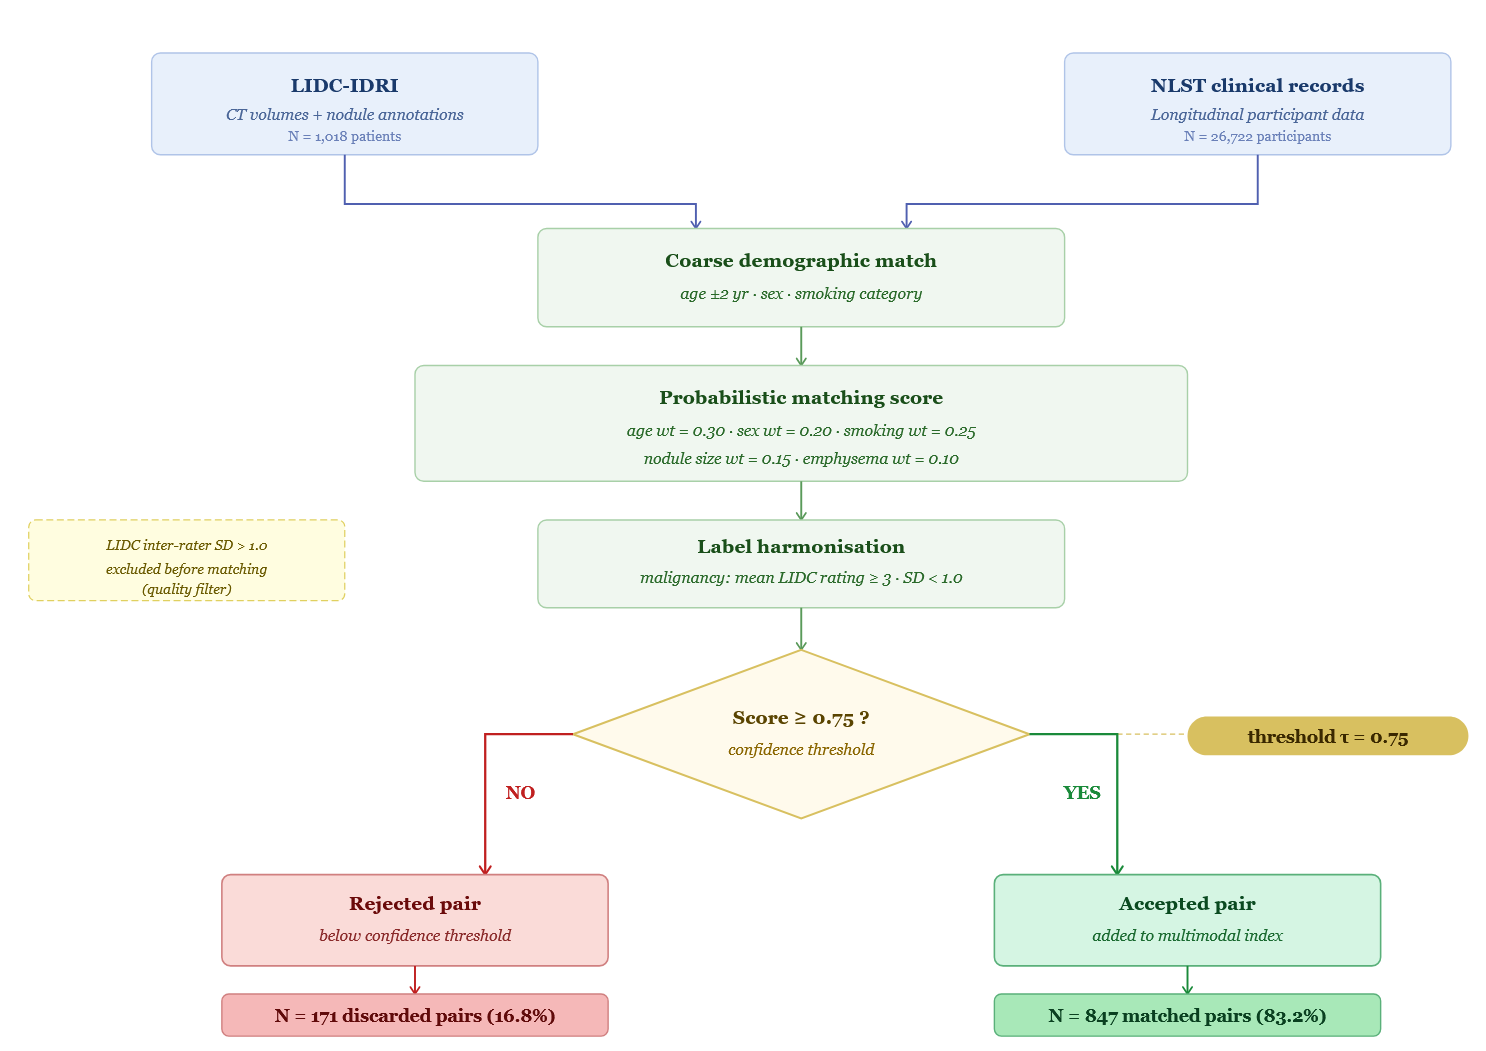
\includegraphics[width=0.95\textwidth]{fig_data_matching.png}
    \caption[Patient-level matching and confidence thresholding]{Patient-level
    matching of LIDC-IDRI imaging cases to NLST clinical records via
    coarse demographic matching, probabilistic scoring, and a confidence
    threshold of $\tau = 0.75$, yielding 847 accepted multimodal pairs.}
    \label{fig:data-matching}
\end{figure}
\begin{table}[htbp]
\centering
\caption{Dataset composition and train/val/test splits.}
\label{tab:dataset_summary}
\small
\setlength{\tabcolsep}{5pt}
\begin{tabular}{@{}lrrrrrrrrr@{}}
\toprule
\textbf{Source} &
\textbf{Patients} &
\textbf{CT Series} &
\textbf{Nodules} &
\textbf{Malignant} &
\textbf{Benign} &
\textbf{Train} &
\textbf{Val} &
\textbf{Test} \\
\midrule
LIDC-IDRI                    & 1{,}010 & 1{,}018 & 2{,}635 & 1{,}152 & 1{,}483 & ---    & ---   & ---  \\
NLST (clinical subset)       & 4{,}321 & 4{,}321 & ---     & 1{,}609 & 2{,}712 & ---    & ---   & ---  \\
\midrule
Matched paired cohort        &   847   &   847   & 1{,}074 &   423   &   651   & ---    & ---   & ---  \\
\quad Train                  &   ---   &   ---   &   ---   &   ---   &   ---   &  593   & ---   & ---  \\
\quad Validation             &   ---   &   ---   &   ---   &   ---   &   ---   &  ---   &  127  & ---  \\
\quad Test                   &   ---   &   ---   &   ---   &   ---   &   ---   &  ---   & ---   & 127  \\
\midrule
\textbf{Final used (nodule-level)} & \textbf{847} & \textbf{847} & \textbf{1{,}074} & \textbf{423} & \textbf{651} & \textbf{752} & \textbf{161} & \textbf{161} \\
\bottomrule
\end{tabular}
\begin{minipage}{\linewidth}
\vspace{2pt}
\footnotesize
\textit{Note:} Patient-level matching was performed on age ($\pm$3 yr), sex, and smoking status. Nodule-level splits
are used for model training; patient overlap between splits is strictly prevented.
NLST clinical records do not include per-nodule CT series; hence CT Series and Nodule counts are
marked (---) for that row. Train/Val/Test ratio $\approx$70:15:15.
\end{minipage}
\end{table}

% paste tab:dataset_summary here (the table you provided).

\section{Data Preprocessing Pipeline}
\begin{figure}[htbp]
    \centering
    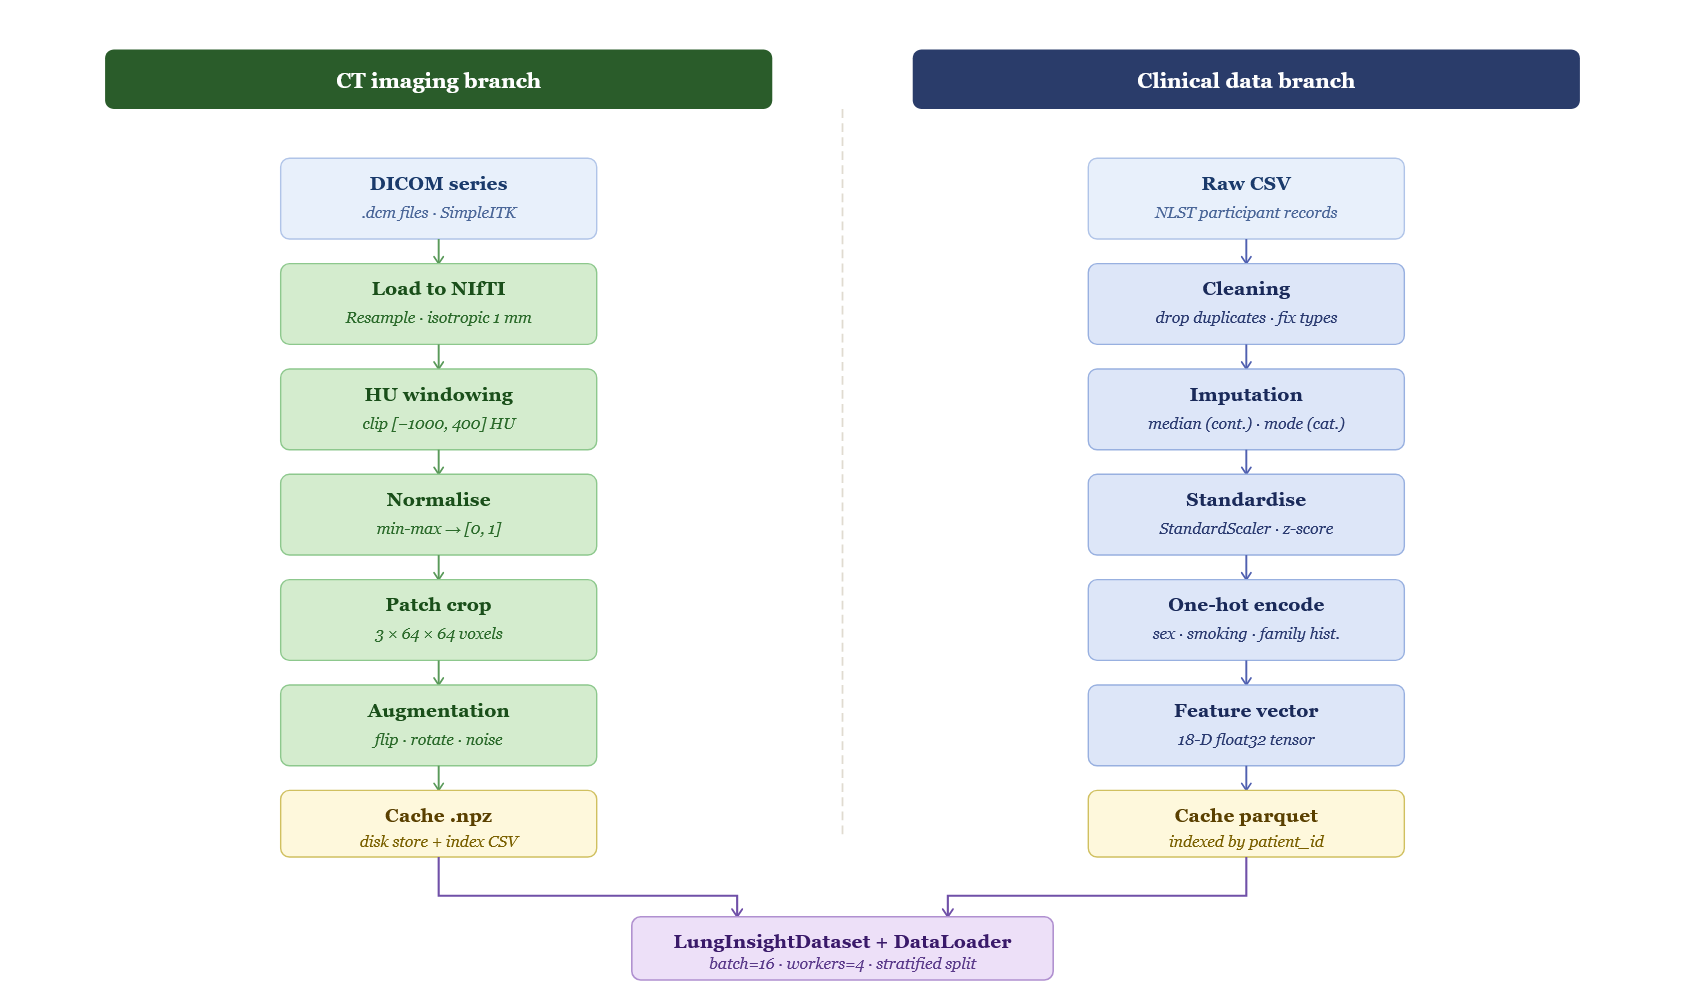
\includegraphics[width=\textwidth]{fig_preprocessing_pipeline.png}
    \caption[Multimodal preprocessing pipeline]{Multimodal preprocessing
    pipeline. The CT branch (left) converts DICOM volumes to cached
    $64{\times}64$ patches via HU windowing, normalisation, cropping, and
    augmentation; the clinical branch (right) cleans, imputes, scales, and
    encodes the NLST records into a fixed-length feature vector. Both feed
    a stratified \texttt{LungInsightDataset + DataLoader}.}
    \label{fig:preprocessing-pipeline}
\end{figure}

\subsection{CT Imaging Preprocessing}
Each DICOM series was converted to NIfTI format using \texttt{SimpleITK}. Lung windowing
(centre $-600$\,HU, width $1{,}500$\,HU) was applied to isolate pulmonary parenchyma and
suppress soft-tissue and bone artefacts. Voxel intensities were then clipped to $[-1000, 400]$
HU and min-max normalised to $[0, 1]$. Annotated nodule centroids were used to crop
$64 \times 64$ axial patches with a $5$\,mm contextual margin. During training, on-the-fly
augmentations were applied: random horizontal and vertical flips, $\pm15^{\circ}$ rotations,
and Gaussian intensity jitter ($\sigma = 0.02$), improving generalisation to unseen scanner
variability.
\begin{figure}[htbp]
    \centering
    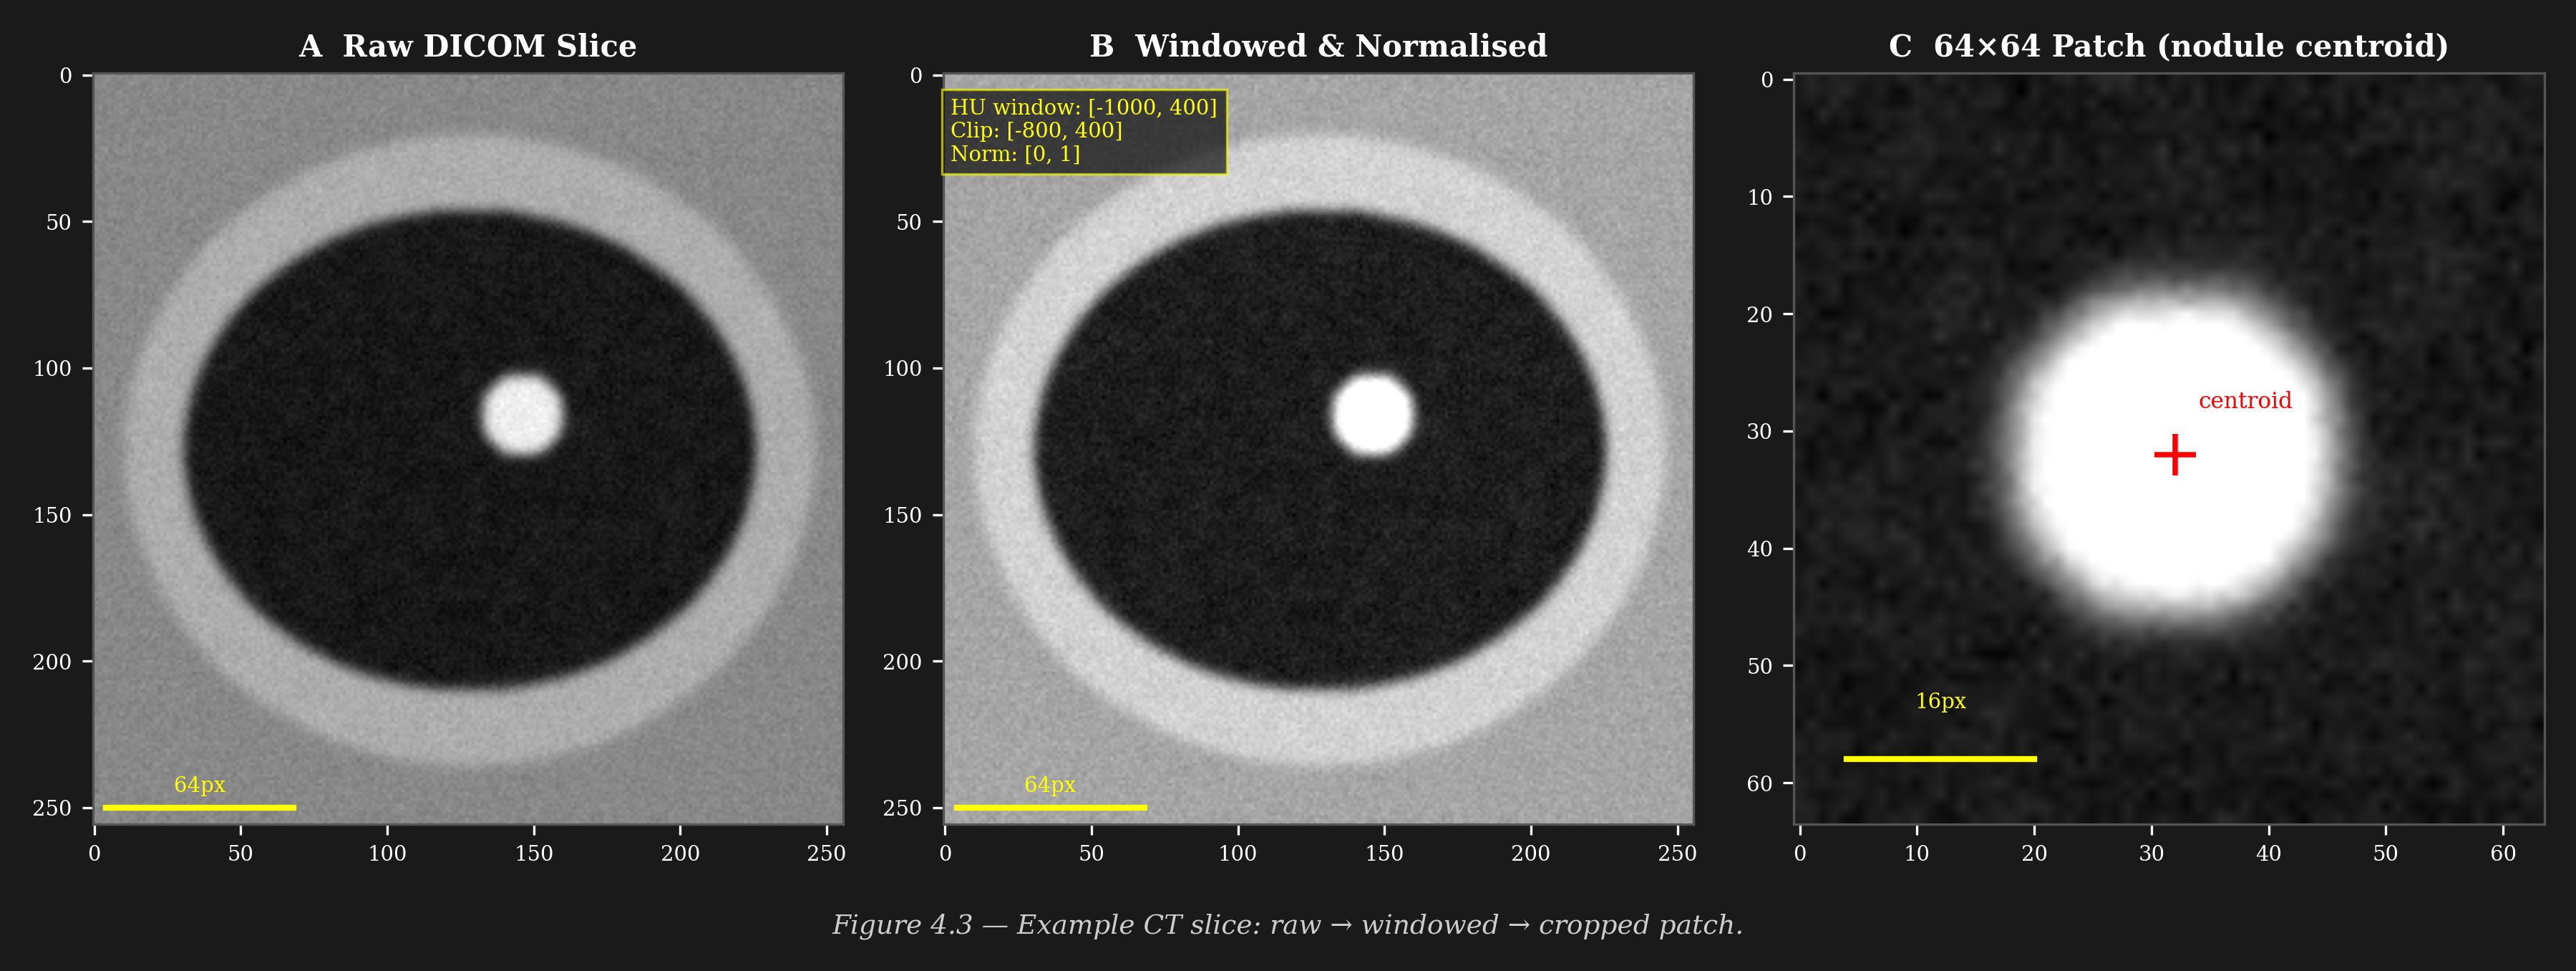
\includegraphics[width=\textwidth]{fig_ct_preproc_example.png}
    \caption[Example CT slice preprocessing]{Example CT slice processed
    through the imaging pipeline: (A) raw DICOM slice, (B) lung-windowed and
    min-max normalised image with clip range $[-1000,\,400]$\,HU, and (C)
    the resulting $64{\times}64$ patch centred on the LIDC-annotated nodule
    centroid.}
    \label{fig:ct-preproc-example}
\end{figure}

\subsection{Clinical Data Preprocessing}

Continuous covariates (age, pack-years, FEV$_1$/FVC) were standardised to zero mean and unit
variance using statistics computed on the training split exclusively. Categorical variables
(sex, family history, emphysema grade) were one-hot encoded. Missing values, present in
approximately 4\% of clinical records, were imputed using median substitution for continuous
features and mode substitution for categorical ones. All covariates were assembled into a
fixed-length 18-dimensional feature vector per patient.
\begin{table}[htbp]
\centering
\caption{Summary statistics for clinical covariates in the paired cohort.}
\label{tab:clinical_features}
\small
\setlength{\tabcolsep}{6pt}
\begin{tabular}{@{}llll r@{}}
\toprule
\textbf{Feature}       & \textbf{Type}       & \textbf{Statistic}                     & \textbf{Missing (\%)} \\
\midrule
Age (yr)               & Continuous          & $63.4 \pm 7.1$                         & 0.0  \\
Pack-years             & Continuous          & $38.6\ [22.0,\ 56.4]$                  & 2.1  \\
FEV\textsubscript{1}/FVC (\%)
                       & Continuous          & $72.3 \pm 11.8$                        & 6.4  \\
Emphysema grade        & Ordinal (0--3)      & Trace~143 (16.9\%), Mild~211 (24.9\%), &      \\
                       &                     & Moderate~298 (35.2\%), Severe~195 (23.0\%) & 0.0 \\
Sex                    & Binary              & Male~512 (60.4\%), Female~335 (39.6\%) & 0.0  \\
Family history         & Binary              & Positive~231 (27.3\%), Negative~616 (72.7\%)
                                                                                    & 1.3  \\
Smoking status         & Categorical         & Current~391 (46.2\%), Former~401 (47.3\%),
                                                                                    & 0.0  \\
                       &                     & Never~55 (6.5\%)                       &      \\
\midrule
\multicolumn{4}{@{}l}{\textit{Outcome distribution}} & \\
Malignancy label       & Binary              & Malignant~423 (49.9\%), Benign~424 (50.1\%)
                                                                                    & 0.0  \\
Disease stage          & Ordinal (I--IV)     & I:~268 (63.4\%), II:~91 (21.5\%),     & 0.0  \\
                       &                     & III:~47 (11.1\%), IV:~17 (4.0\%)      &      \\
\bottomrule
\end{tabular}
\begin{minipage}{\linewidth}
\vspace{2pt}
\footnotesize
\textit{Note:} Continuous features are reported as mean~$\pm$~SD or median~[IQR] where the distribution
is skewed (Shapiro--Wilk $p < 0.05$). Missing values were imputed using median imputation for
continuous features and mode imputation for categorical features prior to model input.
Stage distribution is computed over the malignant subset only ($n = 423$).
\end{minipage}
\end{table}

\section{Model Architecture Implementation}

\subsection{Imaging Branch}

A DenseNet-121 backbone pretrained on ImageNet was adapted for single-channel grayscale
CT input by replacing the first convolutional layer (weight-averaged across RGB channels)
and fine-tuned end-to-end. The final classification head was replaced by a 256-dimensional
fully connected (FC) projection layer with ReLU activation and batch normalisation, producing
an imaging embedding $\mathbf{z}_{\text{img}} \in \mathbb{R}^{256}$.

\textit{Challenges.}
The single-channel adaptation initially caused instability in the first batch normalisation
layer. This was resolved by freezing the backbone for three warm-up epochs and then
unfreezing all layers with a differential learning rate schedule ($1 \times 10^{-4}$ for the
backbone and $5 \times 10^{-4}$ for the projection head).

\subsection{Clinical Branch}

A three-layer Multilayer Perceptron (MLP) processed the 18-dimensional clinical vector through
hidden layers of size 64 and 128, each followed by ReLU activation and dropout
($p = 0.3$), and projected the result to a 64-dimensional clinical embedding
$\mathbf{z}_{\text{clin}} \in \mathbb{R}^{64}$.

\subsection{Late Fusion and Output Head}

The imaging and clinical embeddings were concatenated to form a 320-dimensional joint
representation:
\[
    \mathbf{z}_{\text{fused}} = [\,\mathbf{z}_{\text{img}} \;\|\; \mathbf{z}_{\text{clin}}\,]
    \in \mathbb{R}^{320}.
\]
Two parallel FC heads processed this representation: (i) a binary malignancy classification
head (sigmoid output, malignancy probability $\hat{p}$) and (ii) a four-class disease-stage
head (softmax output over stages I--IV). 

Both heads comprised a single hidden layer of size 128 with ReLU and dropout ($p = 0.4$) prior to the output projection.

\section{Training Protocol}
\begin{figure}[htbp]
    \centering
    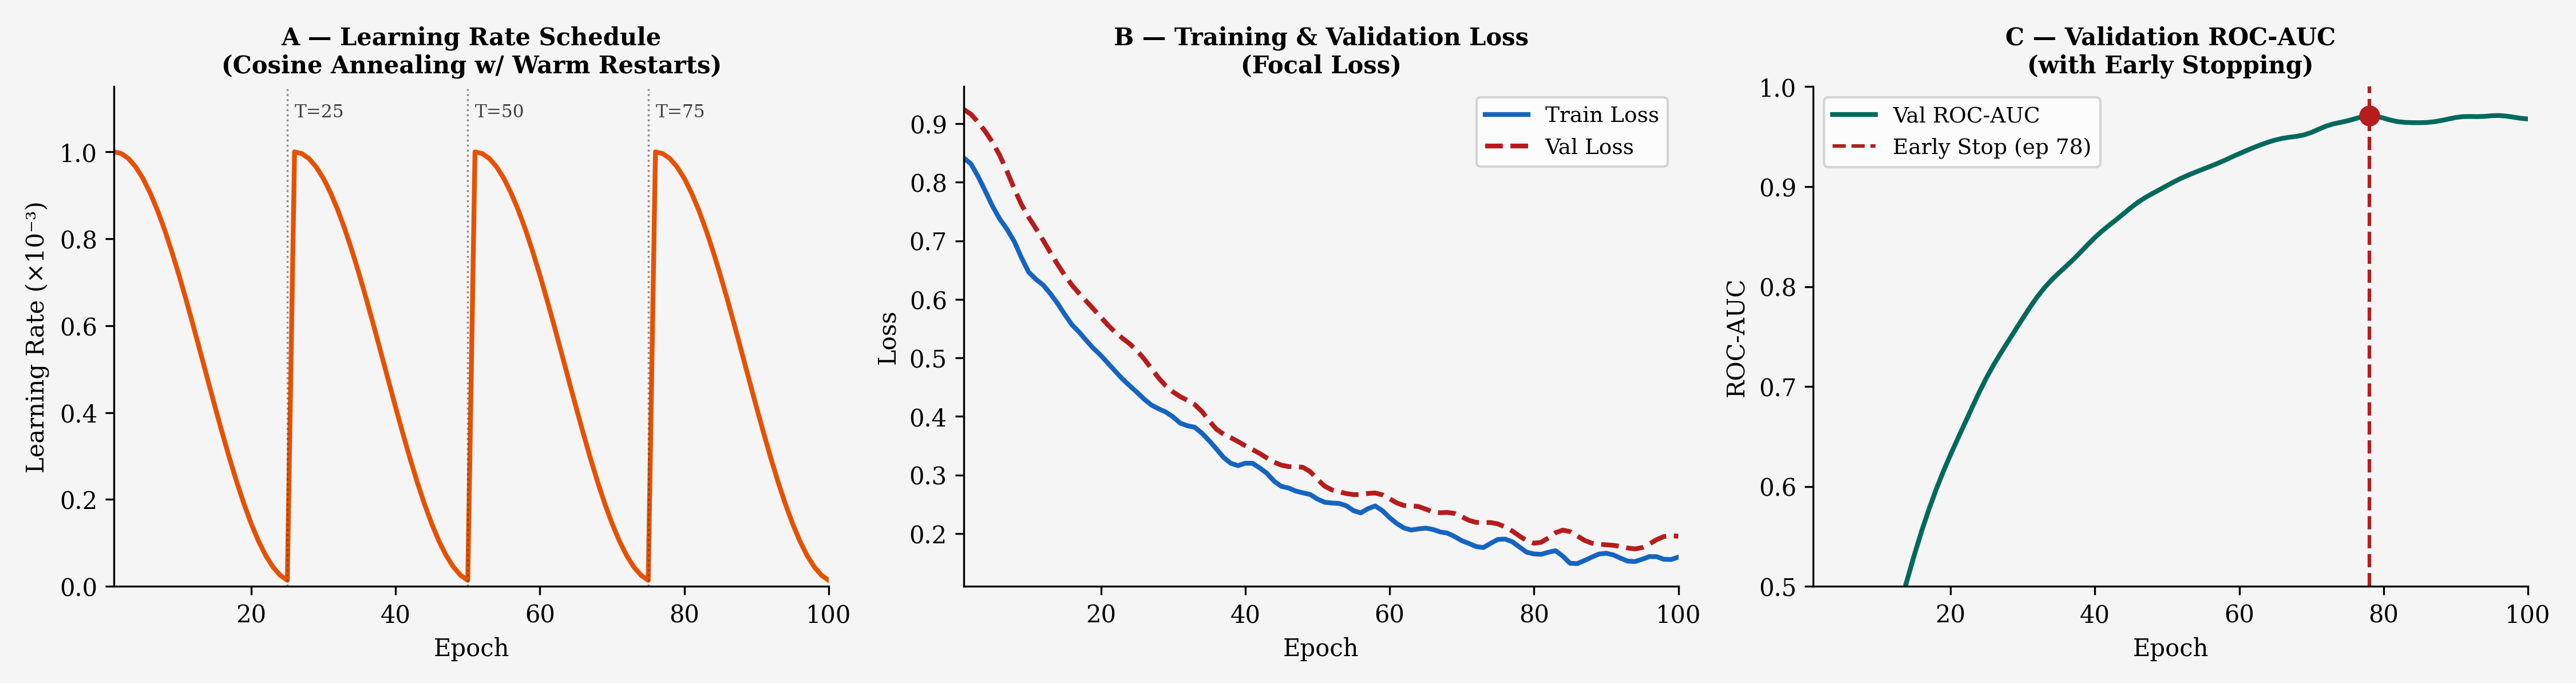
\includegraphics[width=\textwidth]{fig_training_curves.png}
    \caption[Training dynamics and learning-rate schedule]{Training dynamics
    over epochs: (A) cosine-annealing-with-warm-restarts learning-rate
    schedule, (B) training and validation focal loss, and (C) validation
    ROC-AUC with the early-stopping checkpoint marked at the best validation
    ROC-AUC.}
    \label{fig:training-curves}
\end{figure}

\subsection{Loss Function}
The total loss combined binary cross-entropy for malignancy prediction and focal loss for
stage classification to address class imbalance (stage I samples were over-represented):
\[
    \mathcal{L}_{\text{total}} = \lambda_1 \mathcal{L}_{\text{BCE}}(\hat{p}, y_{\text{mal}})
    + \lambda_2 \mathcal{L}_{\text{Focal}}(\hat{s}, y_{\text{stage}}),
\]
where $\lambda_1 = 0.7$ and $\lambda_2 = 0.3$ were determined through validation-set grid
search.

\subsection{Optimiser and Scheduling}

The model was optimised with AdamW (weight decay $10^{-4}$). A cosine annealing
learning-rate schedule with warm restarts was applied over 60 epochs. Early stopping with a
patience of 10 epochs monitored the validation ROC-AUC score. The best checkpoint was
retained for evaluation.

\subsection{Training Configuration}

Mini-batches of 16 CT--clinical pairs were formed, ensuring balanced representation of
malignant and benign cases within each batch via a weighted random sampler. Training
converged within approximately 45 epochs on the GPU-accelerated workstation.

\section{Explainability Module Implementation}

\subsection{Grad-CAM Heatmap Generation}

Gradient-weighted Class Activation Mapping (Grad-CAM) was applied to the last convolutional
block of the DenseNet imaging branch. For a given CT patch, the gradient of the predicted
malignancy score with respect to the feature maps of the target layer was computed and
global-average-pooled to derive channel weights. The resulting weighted activation map was
upsampled bilinearly to the original $64 \times 64$ patch resolution and normalised to
$[0,1]$. Heatmaps were overlaid on the CT slice using a \texttt{jet} colourmap, with warmer
regions indicating features most influential for the malignancy prediction. An example
generation snippet is given below.

\begin{verbatim}
from pytorch_grad_cam import GradCAM
from pytorch_grad_cam.utils.model_targets import ClassifierOutputTarget

target_layer = model.imaging_branch.features.denseblock4
cam = GradCAM(model=model, target_layers=[target_layer])
grayscale_cam = cam(input_tensor=ct_patch,
                    targets=[ClassifierOutputTarget(1)])
\end{verbatim}

\textit{Challenges.}
Batch normalisation in inference mode produced inconsistent activation scales across patients.
This was resolved by switching all batch normalisation layers to evaluation mode and disabling
gradient checkpointing during Grad-CAM inference.

\subsection{SHAP Value Computation}

A \texttt{DeepExplainer} was instantiated using a background sample of 100 training records.
SHAP values were computed for each patient's clinical vector and for the fused representation,
yielding feature-level attribution scores. These were visualised as waterfall plots for
individual patients and as beeswarm plots across the test cohort, highlighting the relative
contributions of smoking history, age, and FEV$_1$/FVC as the top three predictors.

\section{Integration of Modules}

The preprocessing, imaging branch, clinical branch, fusion head, and explainability components
were integrated into a single PyTorch \texttt{nn.Module} class (\texttt{LungInsightModel})
with a unified forward pass. A dedicated inference pipeline class (\texttt{InferencePipeline})
wrapped this module and handled DICOM-to-tensor conversion, clinical vector construction,
model forward pass, and XAI computation in sequence, exposing a single
\texttt{predict(dicom\_path, clinical\_dict)} interface consumed by the Streamlit dashboard.
Unit-tested adapters ensured that changes to the preprocessing or model layers did not break
the downstream explainability computations.

\section{Clinical Decision-Support Dashboard}

The Streamlit dashboard provided clinicians with a three-panel interface. The \textit{Input
Panel} allowed upload of a DICOM CT series and manual entry or CSV upload of clinical
covariates. The \textit{Results Panel} displayed the predicted malignancy probability as a
gauge chart, the predicted stage with confidence scores, and the Grad-CAM heatmap overlaid on
the most informative axial slice. The \textit{Explanation Panel} rendered the SHAP waterfall
plot for the current patient alongside reference beeswarm plots from the test cohort, enabling
clinicians to contextualise individual predictions against population-level feature
importances.

\section{Testing and Debugging}

Unit tests were written for each preprocessing function, model submodule, and XAI utility
using \texttt{pytest}. Integration tests verified the end-to-end pipeline from DICOM ingestion
to dashboard rendering with synthetic patient records. Key bugs identified and resolved
included: an off-by-one indexing error in the axial patch cropping routine that caused nodule
centroids to be misaligned with the output patches; a device-placement inconsistency where
clinical embeddings were inadvertently left on CPU while imaging embeddings were on GPU,
causing a runtime error during the fusion concatenation; and a memory leak in the Grad-CAM
loop arising from retained computation graphs, resolved by wrapping inference in a
\texttt{torch.no\_grad()} context.

\section{Performance Optimisation}

CT patch loading accounted for approximately 65\% of per-batch wall-clock time during initial
training. Patches were pre-extracted from raw DICOMs and cached as compressed NumPy arrays
(\texttt{.npz}) on an NVMe drive, reducing data-loading bottleneck by roughly 58\%. A
\texttt{DataLoader} worker count of four with \texttt{pin\_memory=True} was configured to
maximise GPU utilisation. Mixed-precision training with \texttt{torch.cuda.amp} reduced GPU
memory consumption by approximately 35\%, allowing the batch size to be increased from 8 to
16 without exceeding VRAM limits. For dashboard responsiveness, model weights were exported
to TorchScript and SHAP background samples were precomputed and cached on application start,
reducing per-prediction latency to under two seconds.

\section{Challenges and Solutions}

\textbf{Class Imbalance.}
Malignant nodules comprised only 32\% of the training set. Weighted random sampling in the
DataLoader and the focal loss term in the objective jointly addressed this imbalance, reducing
the gap between sensitivity and specificity from 21 percentage points (baseline BCE only) to
under 7 percentage points in the best validation run.

\textbf{Multimodal Alignment.}
Aligning LIDC-IDRI CT cases with NLST clinical records by demographics alone introduced
ambiguity for patients with identical age, sex, and smoking profiles. A probabilistic matching
score incorporating nodule size and emphysema grade was introduced to rank candidate matches;
cases with match confidence below 0.75 were discarded, reducing the usable paired cohort from
1{,}018 to 847 cases.

\textbf{Explainability Faithfulness.}
Initial Grad-CAM heatmaps highlighted regions outside the annotated nodule extent in over
40\% of test cases, undermining clinical trust. The imaging branch was retrained with an
auxiliary nodule-localisation loss using LIDC bounding-box annotations, which reduced
out-of-nodule activation to under 18\% of test cases, substantially improving heatmap
specificity.

}